\documentclass{article}
\usepackage[utf8]{inputenc} % Permite el uso de caracteres del Español
\usepackage[T1]{fontenc}
\usepackage{hyperref}
\usepackage{graphicx}
\usepackage{wrapfig}
\usepackage{subcaption}


% set font encoding for PDFLaTeX or XeLaTeX
\usepackage{ifxetex}
\ifxetex
  \usepackage{fontspec}
\else
  \usepackage[T1]{fontenc}
  \usepackage[utf8]{inputenc}
  \usepackage{lmodern}
\fi

% used in maketitle
\title{Actividad 5: Preparando datos con ayuda de Emacs}
\author{Melissa Matrecitos Avila}
\date{6 de Marzo de 2018}

% Enable SageTeX to run SageMath code right inside this LaTeX file.
% documentation: http://mirrors.ctan.org/macros/latex/contrib/sagetex/sagetexpackage.pdf
% \usepackage{sagetex}

\begin{document}
\maketitle

\section{Introducción}
El siguiente reporte describe la actividad 5 realizada en el curso de Física Computacional 1, la cual trato sobre la limpieza y análisis de los datos obtenidos en la actividad pasada, enfocados a las variables de CAPE y PW.

A continuación se describirá el significado físico de las variables mencionadas (CAPE y PW), también La preparación del documento para su limpieza en EMACS y su análisis en Python. Por último se presenta una conlcusión sobre la actividad.

\section{Conceptos importantes}
Dos conceptos muy importantes en la actividad fueron el CAPE y PW, de los cuales se hizo un análisis de los datos obtenidos en la estación de Lindenberg, Alemania. Sin embargo antes de pasar a el trabajo con los datos, se debe hablar sobre las variables que se estudiaron.

Las siglas CAPE (Convective Available Potential Energy) hacen referencia a la energia potencial disponible para la convección en un momento dado. CAPE es efectivamente la flotabilidad positiva de un paquete de aire y es un indicador de la inestabilidad atmosférica , lo que lo hace muy valioso para predecir el mal tiempo. Se trata de un parámetro que nos indica cuanta energía está disponible para la convección en caso de que esta se inicie. Por lo tanto, la consulta de este parámetro se tiene que complementar siempre con la lectura de otros campos del modelo que nos permitan determinar la probabilidad de que la convección se inicie.
Es una forma de inestabilidad del fluido que se encuentra en atmósferas térmicamente estratificadas en las que un fluido más frío se superpone a uno más cálido. Como se explica a continuación, cuando una masa de aire es inestable, el elemento de la masa de aire que se desplaza hacia arriba se acelera por la diferencia de presión entre el aire desplazado y el aire ambiente a la altitud (más alta) a la que se desplazó. Esto generalmente crea nubes desarrolladas verticalmente por convección, debido al movimiento ascendente, que eventualmente puede conducir a tormentas eléctricas.

El agua precipitable, o PW por sus siglas en inglés, es la profundidad del agua en una columna de la atmósfera, si toda el agua en esa columna se precipitó como lluvia. Como profundidad, el agua precipitable se mide en milímetros o pulgadas. A menudo abreviado como "TPW" = t otal p recipitable w ater. Hay diferentes técnicas de medición:
\begin{itemize}
\item Un tipo de medición se basa en la medición de la irradiancia solar en dos longitudes de onda, una en una banda de absorción de agua, y la otra no. La columna de agua precipitable se determina usando las irradiancias en estas bandas y la ley de Beer-Lambert .
\item El agua precipitable también se puede calcular mediante la integración de datos de radiosonda ( humedad relativa , presión y temperatura ) en toda la atmósfera .
\item Los datos se pueden ver en un índice Lifted-K. Los números representan pulgadas de agua como se mencionó anteriormente para una ubicación geográfica.
\item Recientemente, se han desarrollado métodos que usan el Sistema de Posicionamiento Global .
\item Se han realizado algunos trabajos para crear relaciones empíricas entre la humedad específica de la superficie y el agua precipitable en base a mediciones localizadas (generalmente un polinomio de segundo a quinto orden). Sin embargo, este método no ha recibido un uso generalizado en parte porque la humedad es una medida local y el agua precipitable es una medición de columna total.
\end{itemize}

\section{Proceso de limpieza y preparación de los datos}
En esta sección se explica el procedimiento utilizado para preparar los datos para su análisis.

Lo primero que se hizo fue crear un script que seleccionaría los renglones con información de la variable CAPE y PW del archivo con los datos de todo el año creado en la actividad 4, y los enviara a un nuevo archivo llamado "df2017CAPE\_PW.csv":
\begin{center}
    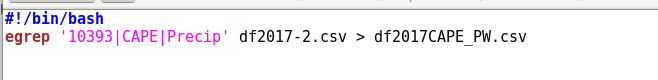
\includegraphics[width=1\textwidth]{FiltroAct4.png}
\end{center}
Transformando el archivo que se muestra a la izquierda en el de la derecha, donde solo esta la información que nos interesa, el cual se copió a la carpeta de Actividad 5:
\begin{center}
    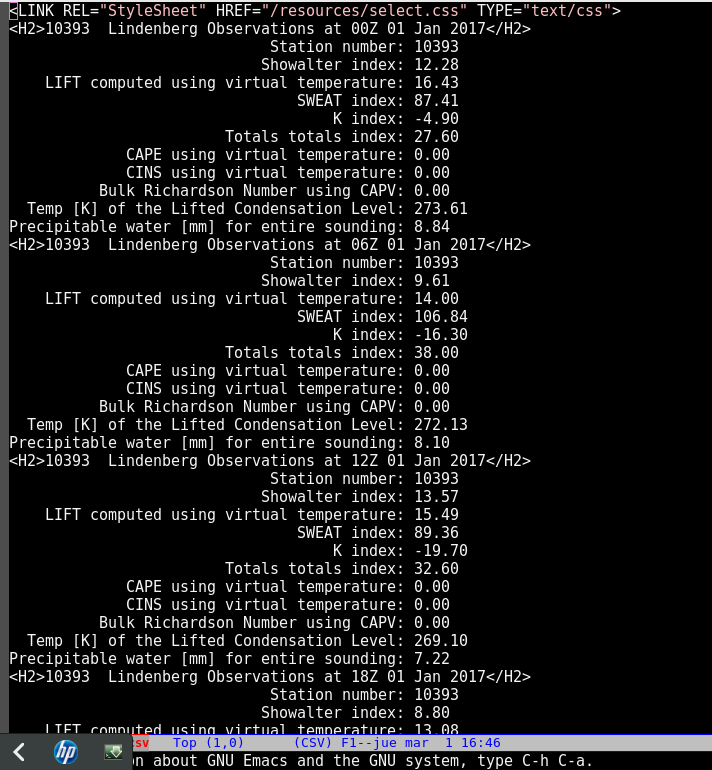
\includegraphics[width=.4\textwidth]{DatosOriginales.png}
     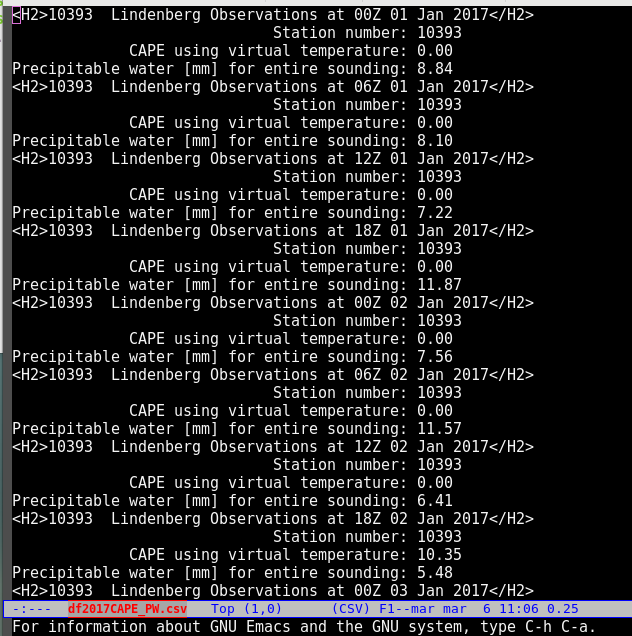
\includegraphics[width=.45\textwidth]{DatosFiltro.png}
\end{center}
Posteriormente se editó el archivo en EMACS para eliminar los datos inecesarios, como la información de la estación y las palabras que describían los datos de cada renglón. Esto se hizo de la siguiente manera:
\begin{enumerate}
\item Se utilizo el comando ctrl y tecla espaciadora para seleccionar el texto a eliminar, desplazándonos con las flechas.
\item Con el comando ctrl y w se eliminaba el texto seleccionado, pero este era enviado a la memoria.
\item Se trajo de vuelta el texto seleccionado con el comando ctrl y y, ya que este vacía la memoria en el lugar indicado.
\item Nos trasladamos al inicio del documento con el comando esc <.
\item Con el comenado esc y \%, el cual es utilizado para remplazar una parte del código por otra, cambiamos el texto guardado previamente en la memoria (ctrl + y) por el que se ocupaba, normalmente se cambiaba por una coma "," o espacios en blanco, dependiendo lo que se quería lograr, por ejemplo par cambiar el mes en la fecha, se cambió el nombre del mes por su número correspondiente.
\item Por último se confirmaban los campos escribiendo "!".
\end{enumerate}
Con este proceso, nos quedaron solo los datos necesarios acomodados por columnas, donde la primera era el lanzamiento, después la fecha, los valores de CAPE y por último los valores de PW. Los datos tenían esta forma:
\begin{center}
    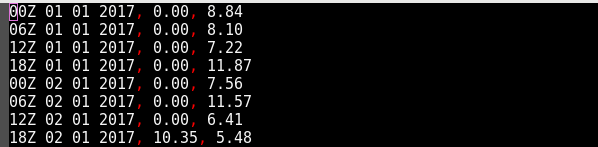
\includegraphics[width=.8\textwidth]{DatosModificados.png}
\end{center}
Por último se separarón los datos en dos archivos, correspondientes al lanzamiento, es decir los 00Z y 12z utilizando el siguiente script:
\begin{center}
    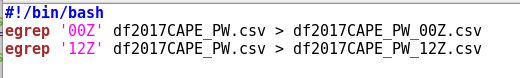
\includegraphics[width=.8\textwidth]{FiltroAct5.png}
\end{center}
El cual selecciona los renglones que tienen 00Z y los envía a un archivo con nombre df2017CAPE\_PW\_00Z.csv, y a los renglones con 12Z los envía al archivo con nombre:df2017CAPE\_PW\_12Z.csv.

A cada uno de los archivos seleccionados, se le eliminó el inicio del renglón, ya que todos los datos correspondían al mismo lanzamiento (00 o 12)

Los archivos quedarón de la siguiente manera, donde el de la izquierda corresponde al 00 y el de la derecha al 12:
\begin{center}
    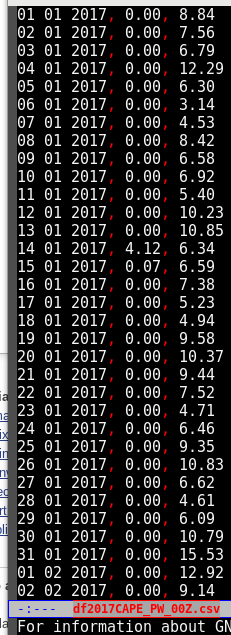
\includegraphics[width=.4\textwidth]{Datos00.png}
    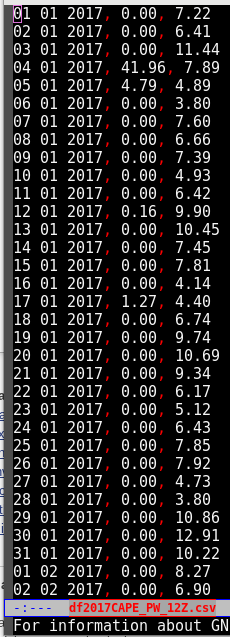
\includegraphics[width=.4\textwidth]{Datos12.png}
\end{center}
\section{Análisis de datos}
A continuación se muestra solo el anális de los datos correspondientes al archivo de los lanzamientos en 00Z, ya que para el archivo de 12Z se hizo lo mismo:
Primeramente se importaron las librerías a utilizar, en cuales había una nueva "datetime" que sirve para dar formato de fecha:
\begin{center}
    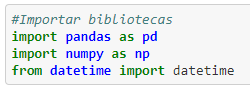
\includegraphics[width=.4\textwidth]{Bibliotecas.PNG}
\end{center}
Posteriormente se colocaron los datos en un dataframe, asignando nombres a la columnas y trasformando la variable CAPE a numérica:
\begin{center}
    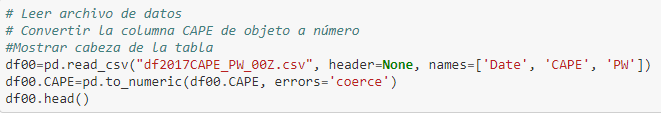
\includegraphics[width=.6\textwidth]{FormatoDatos.PNG}
\end{center}
Quedándonos la siguinete tabla:
\begin{center}
    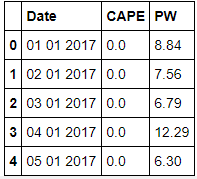
\includegraphics[width=.3\textwidth]{DatosListos.PNG}
\end{center}
Siguiendo con la actividad, se transofromó la columna con nombre Date de tipo objeto a fecha, esto con la nueva biblioteca:
\begin{center}
    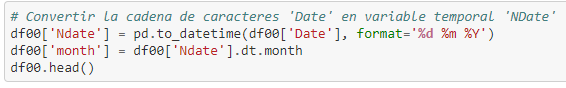
\includegraphics[width=.6\textwidth]{Fecha.PNG}
\end{center}
Dejando los datos listos para hacer las gráficas pertinentes:
\begin{center}
    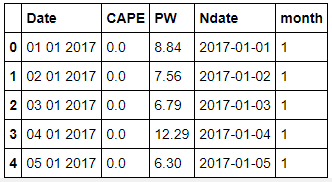
\includegraphics[width=.4\textwidth]{DatosFecha.PNG}
\end{center}
Por último se hicieron las gráficas solicitadas con las siguientes entradas:
\begin{center}
    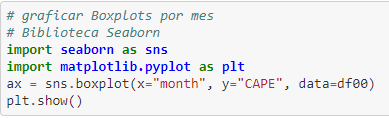
\includegraphics[width=.4\textwidth]{BoxPlotCAPE.PNG}
    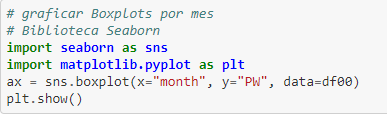
\includegraphics[width=.4\textwidth]{BoxPlotPW.PNG}
    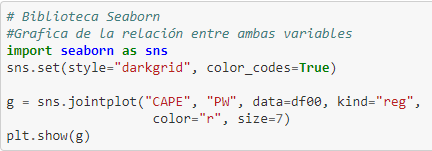
\includegraphics[width=.4\textwidth]{CompararCP.PNG}
    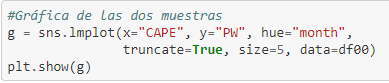
\includegraphics[width=.4\textwidth]{GraficaPareada.PNG}
\end{center}
Las cuales serán explicadas en la sección de "Resultados del análisis".

\section{Resultados del análisis}
A continuación se presentan las gráficas producidas en el análisis de los datos. En todas las gráficas mostradas, las de la izquierda corresponden a los lanzamientos en 00Z y las de la derecha a los lanzamientos en 12Z.
 
\textbf{CAPE}:

Al analizar esta variable se puede decir que a diferencia de la variable CAPE, los valores de PW están alejados del cero, esto se intensifica en los meses de mayo a septiembre, llegando a tener valores desde 20 hasta 35, que corresponde al verano en Alemania. Mientras que en invierno, tiene valores cercanos al 10. Otra diferencia notable entre las variables CAPE y PW es que esta última no tiene tantos valores fuera del rango como la primera.
\begin{center}
    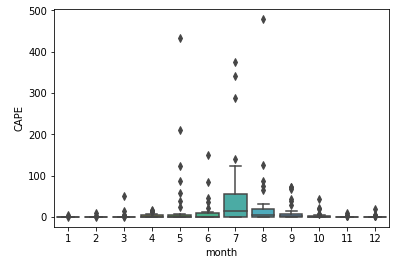
\includegraphics[width=.4\textwidth]{BoxC00.PNG}
    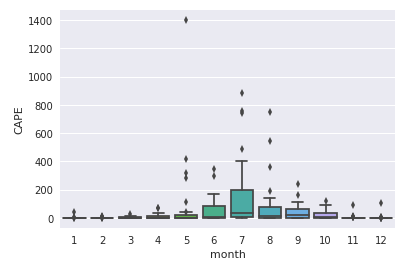
\includegraphics[width=.4\textwidth]{BoxC12.PNG}
\end{center}

\textbf{PW}:

Aquí se muestran los diagramas de caja para los dos lanzamientos con respecto a la variable CAPE. Se puede observar como mantiene valores muy cercanos al cero, excepto por los meses de mayo a agosto, dónde se da un aumento considerable, es decir hay valores fuera del rango.
\begin{center}
    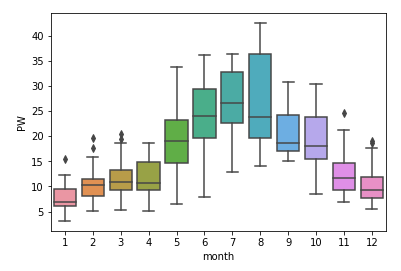
\includegraphics[width=.4\textwidth]{BoxP00.PNG}
    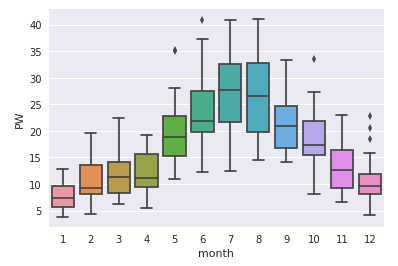
\includegraphics[width=.4\textwidth]{BoxP12.PNG}
\end{center}


\textbf{RELACION PW y CAPE}:

Las siguientes gráficas muestran la distribución de cada variable (arriba la de CAPE y al lado la de PW) y la relación que hay entre ambas. En cuanto a las distribuciones de cada variable no parece haber mucha diferencia entre los lanzamientos, ni la recta que mejor se ajusta. Las gráficas también muestran el coeficiente de correlación de Pearson, el cuál indica que tienen una correlación positiva y al tener valores mayores que cero, se puede decir que pueden estar de algún modo relacionadas linealmente.
\begin{center}
    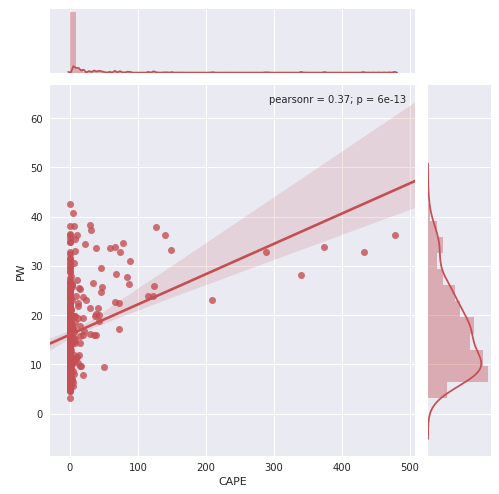
\includegraphics[width=.4\textwidth]{Relacion00.PNG}
    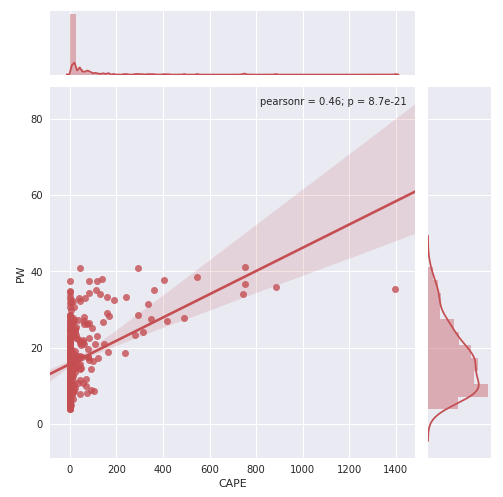
\includegraphics[width=.4\textwidth]{Relacion12.PNG}
\end{center}
\textbf{PAREADOS}:

Las siguientes gráficas muestran los datos pareados, es decir uno en función del otro pero de cada mes, creando una recta de regresión lineal para cada uno. Esto nos puede ayudar a visualizar los cambios conforme pasa el año. Se puede observar tambieén, como la variable CAPE toma valores mayores a los de la variable PW.
\begin{center}
    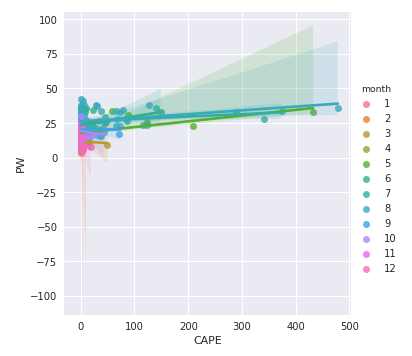
\includegraphics[width=.4\textwidth]{Pareados00.PNG}
    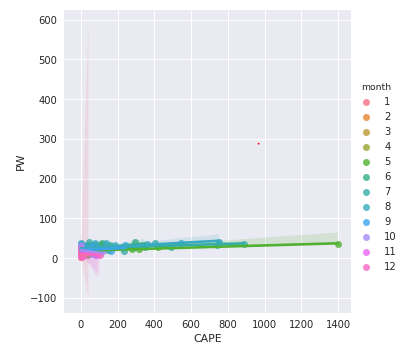
\includegraphics[width=.4\textwidth]{Pareados12.PNG}
\end{center}

\section{Conclusión}
Como se ha mencionado en las actividades pasadas, el proceso de limpieza y preparación de datos es lo más laborioso, incluso más que su propio análisis. Es por esto que el aprender a utilizar EMACS para el trabajo de datos es de suma importancia ya que facilita el trabajo, haciendo que este sea menos pesado. Otro aspecto importante es la automatización de los procesos, ya que permite mayor rapidez en la limpieza de los archivos.

Respecto al análisis de los datos en Python, las nuevas bibliotecas utilizadas fueron de gran ayuda para visualizar la relación que había entre los datos, facilitando de esta manera, la interpretación de la información.

\section{Bibliografía}
\begin{itemize}
\item CAPE y algunas nociones básicas sobre convección atmosférica. (2018). Meteoillesbalears.com. Recuperado el 5 de Marzo de 2018, de \url{http://www.meteoillesbalears.com/?p=623}
\item Precipitable water. (2018). En.wikipedia.org. Recuperado el 5 de Marzo de 2018, de \url{https://en.wikipedia.org/wiki/Precipitable_water}
\item Convective available potential energy. (2018). En.wikipedia.org. Recuperado el 5 de Marzo de 2018, de \url{https://en.wikipedia.org/wiki/Convective_available_potential_energy}
\end{itemize}

\section{Apendice}
\begin{enumerate}
\item¿Cómo se te hizo esta actividad? ¿Compleja, Difícil, Sencilla?
Una vez qu entendí que era lo que estaba haciendo y para que lo hacía, me pareció muy sencilla.

\item¿Qué te llamó más la atención?
Las funciones de EMACS enfocadas ala limpieza de datos, ya que antes solo lo había usado como editor de texto, sin saber todo lo que podía hacer en este.

\item¿Qué parte fue la que menos te interesó hacer?
Todo me pareció interesante, ya que fue como un resumen de las actividades pasadas pero una manera más eficiente.

\item¿Cómo mejorarías esta actividad? ¿Qué le faltó? ¿Qué sobró?
Me pareció una practica muy completa, que me sirvió para reforzar lo visto en actividades pasadas.

\item¿Hasta este punto, que te parece el uso de Jupyter para programar en Python?
Me parece un ambiente muy amigable y muy util para el análisis de los datos, sobre todo por las bibliotecas con las que se trabajó.

\end{enumerate}

\end{document}
